\subsection{Kontrola wersji}

Jedną z najważniejszych części CI/CD są systemy kontroli wersji. 
W przypadku współpracy nad kilkuosobowym projektem, ogromnym rozwiązaniem 
we wiodącej firmie czy nawet pracując samemu - możliwość cofnięcia konkretnych zmian, 
sprawdzenia historii poprawek aby poznać lub przypomnieć sobie ich kontekst, 
jak również aby sprawdzić w jaki sposób coś działało wcześniej - każdy z tych scenariuszy 
mógłby być zastąpiony zwykłą kopią zapasową. 
Ze względu na optymalizację czasowo-kosztową (szybkość działania, 
wygodę obsługi, optymalizację zajmowanego miejsca) znacznie lepszym systemem są dedykowane 
rozwiązania, takie jak Subversion (SVN), CVS czy opisany niżej (prawdopodobnie najpopularniejszy) Git.

W dużym skrócie, Git jest systemem kontroli wersji, charakteryzujący się:
\paragraph{Rozproszeniem repozytoriów}
Pobierając aktualną wersję kodu, najczęściej wykonujemy również pełne sklonowanie repozytorium, 
co częściowo uodparnia system na ewentualne utraty efektów pracy przez awarie sprzętowe lub pomyłki.
Możemy również cofać się w historii wersji bez wielokrotnego kontaktowania się z serwerem.

\paragraph{Zaoszczędzenie przestrzeni dyskowej}
Mechanizm różnicowego przechowywania danych pozwala na zmniejszenie rozmiaru plików, 
wciąż zachowując możliwość dostępu do ich wcześniejszych wersji.
Zamiast wielokrotnie nieznacznie zmieniony plik w całości, wystarczy notować w którym miejscu 
wprowadziliśmy jakie zmiany. Jest to metoda mniej wydajna obliczeniowo, ponieważ każde cofnięcie się 
o konkretną ilość wersji prowadzi do inkrementacyjnego odtworzenia informacji, 
ale jest to na tyle mały narzut pracy względem zaoszczędzonej przestrzeni dyskowej, że w połączeniu 
z prędkością aktualnych komputerów jest to bardziej opłacalna metoda~\cprotect\footnote{%
    Oczywiście istnieją specjalne mechanizmy pozwalające na optymalizację tego zachowania, 
    dobrym punktem wyjścia jest \verb|git maintenance|~\cite{gitMaintenance}}.

\paragraph{Uproszczeniem pracy zespołowej}
System branchy (z ang. gałęzi, odgałęzień) pozwala na odesparowanie konkretnych funkcjonalności, 
podzielenia fragmentów pracy na etapy, jak również na wygodne odseparowanie środowisk pracy deweloperów.
Nie każda osoba musi pobierać wszystkie odgałęzienia, nie mamy ograniczeń ilościowych lub wielkościowych 
jeżeli chodzi o wprowadzane zmiany. Możemy zacząć nad czymś pracować, ale jeżeli będziemy chcieli tymczasowo 
wstrzymać lub porzucić prace, możemy niemalże bez konsekwencji odłożyć je na później i zacząć wdrażać 
inne funkcjonalności.\\%
Po zakończeniu pracy w danym branchu, możemy z powrotem włączyć go do współdzielonej części - następuje 
wtedy specjalne porównanie zmian, które w większości wypadków pozwala na automatyczne ich połączenie, 
a w razie bardziej skomplikowanych niuansów łatwo rozwiejemy wątpliwości w specjalnym narzędziu.

\subsubsection{Integracje międzysystemowe}
Platformy oferujące usługi hostingowe (takie jak zastosowany w tej pracy GitHub~\cite{github}) oferują 
ogromną gamę integracji najróżniejszych narzędzi i systemów - począwszy od możliwości importu 
repozytoriów, nienadzorowanego udostępniania jego zawartości, powiadomienia o zmianach przez najróżniejsze 
kanały informacyjne (WebHooki, RSS, powiadomienia i e-maile), jak również dostęp do wielu innych 
funkcjonalności jak narzędzia upraszczające i formalizujące kontakt z zespołem 
lub podstronie wydawczej, takiej jak GitHub Releases~\cite{githubReleases}.

GitHub Releases to specjalny mechanizm, pozwalający na opublikowanie gotowych rozwiązań, dostępnych do 
pobrania w gotowej do użytku formie. Na rysunku~\ref{img:githubReleases_sample} możemy zobaczyć 
przykładowe wydanie wersji programu - zawiera tytuł (lub w tym przypadku numer wersji), listę zmian 
oraz co najważniejsze skompilowane pliki wraz z ich ekwiwalentnym kodem źródłowym.
\begin{figure}[ht]
    \centering
    \frame{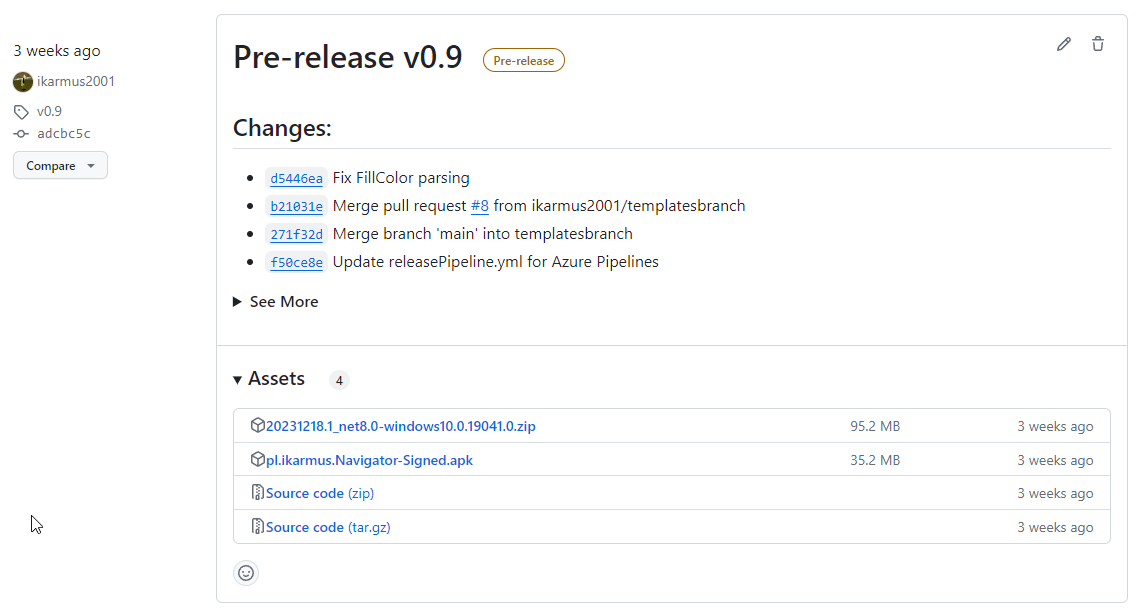
\includegraphics[width=0.9\textwidth]{githubReleases_sample.png}}
    \caption{Przykładowe wydanie aplikacji w GitHub Releases}
    \label{img:githubReleases_sample}
\end{figure}

W moim projekcie skorzystałem również z opcji triggerów (ang. wyzwalaczy), które powiadamiają 
połączone usługi o zmianach w kodzie. \\%
Wysłanie kolejnego commita na określony branch powiadamia 
Azure o tym fakcie, co skutkuje zakolejkowaniem nowego uruchomienia pipeline'a.